\documentclass[12pt]{exam}
\usepackage[utf8]{inputenc}
\usepackage[a4paper,top=20mm]{geometry}
\usepackage[fleqn]{mathtools}
\usepackage{xcolor}
\usepackage{hyperref}
\usepackage{dirtytalk}
\usepackage{setspace}
\usepackage{amsfonts}
\usepackage{graphics}
\usepackage{tikz}
\graphicspath{ {./images/} }
\usepackage{graphicx}
\usepackage{amssymb}
\usepackage{amsmath}
\usepackage{parskip}
\usepackage{caption}
\usepackage{commath}
\usetikzlibrary{graphs}
\newcommand\ddfrac[2]{\frac{\displaystyle #1}{\displaystyle #2}}
\newcommand*\circled[1]{\tikz[baseline=(char.base)]{
            \node[shape=circle,draw,inner sep=2pt] (char) {#1};}}
\DeclareMathOperator{\Deg}{deg}
\title{ZPC-30}
\author{Bikramjyot, Farhan, Ishaan, Rachit}
\date{\today}
\doublespacing

\begin{document}

\captionsetup{font=footnotesize}

\maketitle
\rule{\textwidth}{1pt}
\printanswers

\title{\textbf{\underline{\fontsize{18}{12}\selectfont Instructions}}}\\
Please read the following instructions carefully before proceeding further:\\
\begin{enumerate}
\item The test is of 2 hours. It will end \textit{sharp} at \textbf{8:00 pm}.
\item Relevant reading material for all the questions has been provided in the document itself.
\item If you are stuck on a question that you cannot figure out, move on. Nothing good ever comes out of being hung up on something.
\item Please feel free to contact the invigilators in case of any queries.
\item We will provide hints to questions in the last hour, depending on the participation and responses.
\item All the best. GL HF :)\\
\end{enumerate}
\bigskip
\maketitle
\newpage
\title{\begin{center}\textbf{\underline{\fontsize{16}{12}\selectfont CHROMATIC POLYNOMIALS}}\end{center}}

\textbf{Note:} We will only be working with simple undirected graphs (graphs which do not contain duplicate edges or self-loops).

\section{Graphs}

A graph can be defined as a pair $G=(V,E)$.

The elements of the set $V$ are called the \emph{vertices} of the graph, and the elements of the set $E$ are called the \emph{edges} of the graph. Every element of $E$ is a 2-element subset of $V$.  

The following are examples of graphs, represented both diagrammatically and in notation,

\begin{figure}[h]

    \centering
    
    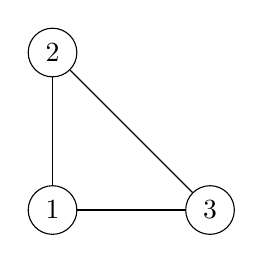
\begin{tikzpicture}[scale=2,auto=center,every node/.style={circle,draw=black}]
        \node (1) at (0,0) {1};
        \node (2) at (0,1) {2};
        \node (3) at (1,0) {3};

        \draw (1) -- (2);
        \draw (2) -- (3);
        \draw (3) -- (1);
    \end{tikzpicture}

    \caption{Graph $G = (E,V)$ where $E = \{1,2,3\}$ \\ and $V=\{\{1,2\},\{2,3\},\{3,1\}\}$}
    
\end{figure}

\begin{figure}[h]
    \centering
    
    \begin{tikzpicture}[scale=2,auto=center,every node/.style={circle,draw=black}]
        \node (1) at (0,0) {a};
        \node (2) at (1,0) {b};
        \node (3) at (0,1) {c};
        \node (4) at (-0.75,-0.75) {d};

        \draw (1) -- (4);
    \end{tikzpicture}

    \caption{Graph $G = (V,E)$ where $V = \{a,b,c,d\}$ and $E = \{\{a,d\}\}$}
    
\end{figure}

\newpage

Note that vertices of a graph may also be unlabeled:

\begin{figure}[h]
    \centering

    \begin{tikzpicture}[scale=2,auto=center,every node/.style={circle,draw=black}]
        \node (1) at (0,0) {};
        \node (2) at (0, 1) {};
        \node (3) at (0.70, -0.70) {};
        \node (4) at (-0.70,-0.70) {};

        \draw (1) -- (2);
        \draw (1) -- (3);
        \draw (1) -- (4);
    \end{tikzpicture}

    \caption{A graph without labels.}
    
\end{figure}

If we want to represent this graph formally, we can simply assign our own labels to nodes.

As we can see, graphs are useful in scenarios where we need to represent a set of objects with a sense of \say{connection} between some pairs of those objects.

We could, for example, make a graph whose vertices are the set of people at a party, and an edge between two vertices could represent pairs of people who already know each other.

Now we come to a popular area of research in graph theory, graph colorings.

\section {Graph colorings}

A \emph{coloring} of a graph $G=(V,E)$ is a mapping $f:V \rightarrow C$ where $C$ is a set of symbols or objects known as \emph{colors}, where any two vertices sharing an edge must not be mapped to same \emph{color}. More formally, for all $\{v_1, v_2\} \in E, f(v_1) \neq f(v_2)$.

Let's consider an example. 

Suppose we have a group of $n$ students sitting in a circle. We want to assign each student a \emph{team}, \textbf{red} (denoted by $R$) or \textbf{blue} (denoted by $B$), such that no two students sitting next to each other share the same team.

For any given $n$, we can represent this scenario as a graph; more specifically $C_n$, the  \textbf{circular graph} with $n$ nodes.

Consider $n=8$.

\begin{figure}[h]

    \centering
    
    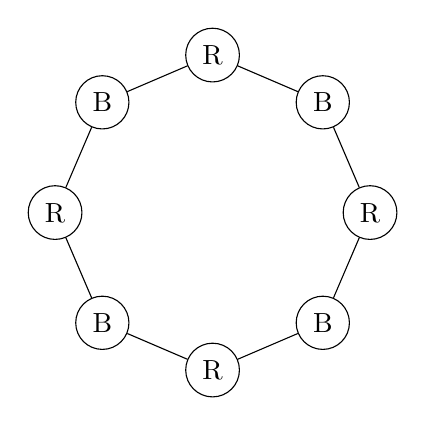
\begin{tikzpicture}[scale=1,auto=center,every node/.style={circle,draw=black}]
        \node (1) at (2,0) {R};
        \node (2) at (1.4,1.4) {B};
        \node (3) at (0,2) {R};
        \node (4) at (-1.4, 1.4) {B};
        \node (5) at (-2, 0) {R};
        \node (6) at (-1.4,-1.4) {B};
        \node (7) at (0, -2) {R};
        \node (8) at (1.4, -1.4) {B};
        \draw (1) -- (2);
        \draw (2) -- (3);
        \draw (3) -- (4);
        \draw (4) -- (5);
        \draw (5) -- (6);
        \draw (6) -- (7);
        \draw (7) -- (8);
        \draw (8) -- (1);
    \end{tikzpicture}

    \caption{A 2-coloring of the graph $C_8$.}
    
\end{figure}

The $n=2k$ (even cycles) case is quite easy. We simply color one node red or blue, and keep filling all adjacent nodes with the opposite color.

\textbf{However, when $n = 2k+1$ (odd cycles), it is actually impossible to make a valid coloring using 2 colors.}

\begin{figure}[h]

    \centering
    
    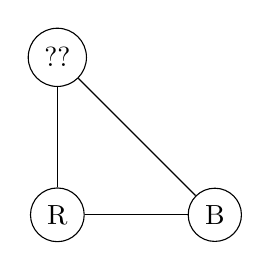
\begin{tikzpicture}[scale=2,auto=center,every node/.style={circle,draw=black}]
        \node (1) at (0,0) {R};
        \node (2) at (1,0) {B};
        \node (3) at (0,1) {??};
        \draw (1) -- (2);
        \draw (2) -- (3);
        \draw (3) -- (1);
    \end{tikzpicture}

    \caption{There exists no 2-coloring of graph $C_3$.}
    
\end{figure}

As we can see in the figure above, an odd cycle of length 3 cannot be colored using 2 colors.

\textbf{Convince yourself that no odd cycle can have a coloring with 2 colors.}

However, all odd cycles can be colored using 3 colors. Let's introduce another color, $G$. An odd cycle of length 5 can be colored using $R$, $B$ and $G$ as follows, 

\newpage 

\begin{figure}[h]

    \centering
    
    \begin{tikzpicture}[scale=2,auto=center,every node/.style={circle,draw=black}]
        \node (1) at (0,2) {R};
        \node (2) at (1,1) {B};
        \node (3) at (1,-1) {\textbf{G}};
        \node (4) at (-1, -1) {R};
        \node (5) at (-1, 1) {B};
        \draw (1) -- (2);
        \draw (2) -- (3);
        \draw (3) -- (4);
        \draw (4) -- (5);
        \draw (5) -- (1);
    \end{tikzpicture}

    \caption{A 3-coloring of graph $C_5$.}
    
\end{figure}

\section{Chromatic Number}

The minimum number of colors required to make a valid coloring of a graph $G$ is called the \textbf{chromatic number} of $G$, often denoted as $\chi(G)$.

As we have seen, graphs of type $C_{2k+1}$ (odd cycles) have chromatic number 3 ($\chi(C_{2k+1}) = 3$ for all $k$) and graphs of type $C_{2k}$ (even cycles) have chromatic number 2 ($\chi({C_{2k}}) = 2$ for all $k$).

For example, consider the complete graph on $n$ vertices, $K_n$, in which all pairs of nodes have an edge between each other.

$K_5$ is illustrated below:

\newpage

\begin{figure}[h]

    \centering
    
    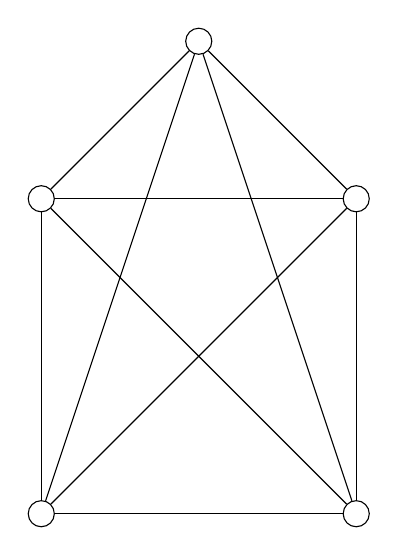
\begin{tikzpicture}[scale=2,auto=center,every node/.style={circle,draw=black}]
        \node (1) at (0,2) {};
        \node (2) at (1,1) {};
        \node (3) at (1,-1) {};
        \node (4) at (-1, -1) {};
        \node (5) at (-1, 1) {};
        \draw (1) -- (2);
        \draw (1) -- (3);
        \draw (1) -- (4);
        \draw (2) -- (3);
        \draw (2) -- (4);
        \draw (2) -- (5);
        \draw (3) -- (4);
        \draw (3) -- (5);
        \draw (4) -- (5);
        \draw (5) -- (1);
    \end{tikzpicture}

    \caption{The complete graph of 5 vertices, $K_5$.}
    
\end{figure}

Graphs of type $K_n$ have chromatic number $n$, because all the nodes need to be of different colors.

\textbf{Note that if a graph can be colored using $k$ colors, it can also be colored using $k+1$ or $k+2$ (and so on) colors, because using all colors in the set of colors is not mandatory. Each node must have at least one color, so we cannot go lower than the chromatic number. Therefore, every valid $k$-coloring of a graph is also a valid $l$-coloring where $l>k$}. 

\section{Chromatic Polynomials}

What if we were given a graph $G$, and we wanted to construct a function which gives us the number of $k$-colorings of $G$ for any given $k$?

Turns out we have a solution to this, called the \textbf{chromatic polynomial} of the graph $G$.

The chromatic polynomial $p_G(\lambda)$ is a polynomial function in $\lambda$:
\begin{gather*}
    p_G(\lambda) = \lambda^n + a_1 \lambda^{n-1} + a_2\lambda^{n-2} + \cdots + a_n
\end{gather*}

where $p_G(k)$ is the number of valid $k$-colorings of the graph $G$.

Consider the example of $E_n$, the graph with $n$ nodes and \emph{no edges}. What is the chromatic polynomial of this graph?

Suppose we have $k$ colors. Each node has $k$ choices of colors independent of each other, since there are no edges. So the number of $k$-colorings of $E_n$ is $k^n$.

So, the chromatic polynomial for $E_n$ is $p_{E_n}(\lambda) = \lambda^n$.

Now, consider the opposite of this graph, the complete graph $K_n$ which we discussed earlier. \textbf{The chromatic polynomial of the complete graph $K_n$ is:}
\begin{gather*}
    p_{K_n}(\lambda) = \lambda(\lambda - 1)(\lambda - 2)\cdots(\lambda - n + 1)
\end{gather*}

Here's how we came up with the chromatic polynomial of $K_n$:

\begin{itemize}
    \item Since for $k=1,2,\cdots,n-1$ there are no valid colorings, those $k$ must be zeroes of the polynomial.
    \item Suppose $k \geq n$. Suppose we color the first node with color $c_1$ with $\lambda$ choices. Then, the next node must be colored $c_2$ with $\lambda - 1$ choices, and so on, which gives us the expression above that \emph{happens to have} numbers from 1 to $n-1$ as its zeroes.  
\end{itemize}

We'll also look at a more formal and objective way to calculate the chromatic polynomial of a graph in the upcoming section.

\textbf{Make sure you understand everything by this point, ok? I know it's a lot to take in if you have never dabbled in graph theory, but feel encouraged to ask a coordinator anything you're unsure about. After all, the point is to learn something and have fun doing it!}

\section{Deletion-Contraction Algorithm}

The deletion-contraction algorithm is an algorithm to compute the chromatic polynomial of a given graph.

Before we cover the formula, we need to introduce 2 new graph operations, \textbf{edge deletion} and \textbf{edge contraction}.

\subsection*{Edge deletion}

Suppose $G = (V, E)$ is a graph with a non-empty edge set. Let $e \in E$ be  an edge of the graph $G$. The deletion $(G - e)$ is defined as the graph $G = (V, E - e)$.

Essentially, we are removing the edge $e$ from the graph without affecting any other edges.

\begin{figure}[h]

    \centering
    
    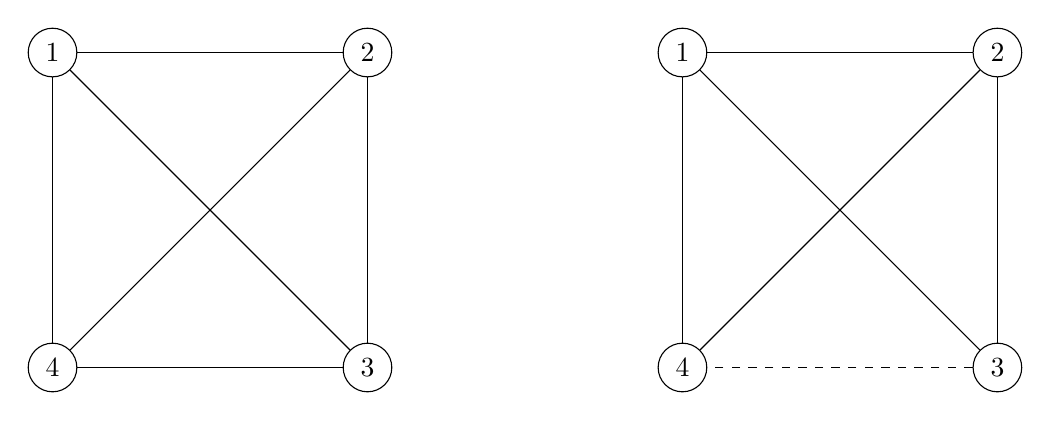
\begin{tikzpicture}[scale=2,auto=center,every node/.style={circle,draw=black}]
        \node (2) at (-1,1) {2};
        \node (1) at (-3,1) {1};
        \node (3) at (-1,-1) {3};
        \node (4) at (-3, -1) {4};

        \draw (1) -- (2);
        \draw (2) -- (3);
        \draw (3) -- (1);
        \draw (3) -- (4);
        \draw (4) -- (1);
        \draw (2) -- (4);

        \node (6) at (3,1) {2};
        \node (5) at (1,1) {1};
        \node (7) at (3,-1) {3};
        \node (8) at (1, -1) {4};

        \draw (5) -- (6);
        \draw (5) -- (7);
        \draw (6) -- (8);
        \draw (5) -- (8);
        \draw (6) -- (7);
        \draw (7) -- (8) [dashed];
    \end{tikzpicture}

    \caption{On the left: Graph $K_4$. On the right: $(K_4 - \{3,4\})$. (To be painfully precise: \{3,4\} is not contained in the edge set of the right graph.)}
    
\end{figure}


\subsection*{Edge contraction}

Suppose $G = (V, E)$ is a graph with a non-empty edge set. Let $e \in E$ be  an edge of the graph $G$. The contraction $(G \backslash e)$ can be seen as \say{merging} the two vertices $v_1$ and $v_2$ connected by the edge into one vertex as follows:

\begin{enumerate}
    \item The edge ${v_1, v_2}$ is removed from the edge set.
    \item Any edge $e'$ where $v_2 \in e'$ is converted to $((e' - \{v_2\}) \cup v_1)$.
    \item The node $v_2$ is removed from the graph.
\end{enumerate}

\begin{figure}[h]

    \centering
    
    \begin{tikzpicture}[scale=2,auto=center,every node/.style={circle,draw=black}]
        \node (1) at (-2,2) {1};
        \node (2) at (-1,1) {2};
        \node (3) at (-1,-1) {3};
        \node (4) at (-3, -1) {4};
        \node (5) at (-3, 1) {5};
        \draw (1) -- (3);
        \draw (2) -- (3);
        \draw (4) -- (1);
        \draw (2) -- (5);
        \draw (4) -- (5);
        \draw (5) -- (1);
        \node (1) at (2,2) {1};
        \node (2) at (3,1) {2};
        \node (4) at (2, -1) {4};
        \node (5) at (1, 1) {5};
        \draw (1) -- (4);
        \draw (2) -- (4);
        \draw (4) -- (1);
        \draw (2) -- (5);
        \draw (4) -- (5);
        \draw (5) -- (1);
    \end{tikzpicture}

    \caption{On the left, an arbitrary graph $G$. On the right, $(G \backslash \{3,4\})$. Nodes 3 and 4 are merged into 4.}
    
\end{figure}

\subsection*{Statement of the Deletion-Contraction Algorithm}

Suppose we need to calculate the chromatic polynomial of a graph $G = (V, E)$. 

If $E(G) = \emptyset$, then $G$ is the empty graph of $\abs{V}$ vertices, and its chromatic polynomial is $p_G(\lambda) = \lambda^{\abs{V}}$. 

Otherwise, we inductively calculate the chromatic polynomial of $G$ as follows:

\begin{gather*}
    p_G(\lambda) = p_{G - e}(\lambda) - p_{G \backslash e}(\lambda)
\end{gather*}


Where $e$ is any edge in $G$.

\subsection*{Intuition behind the formula}

\begin{itemize}
    \item Any valid coloring of $G$ is a valid coloring of $(G - e)$ (convince yourself why.)
    \item The only colorings of $(G-e)$ which are not valid in $G$ are the colorings of $(G \backslash e)$, when the color of $v_1$ and $v_2$ is the same in $G - e$. (convince yourself why.)
\end{itemize}

\newcommand{\marksA}[1]{\hfill\makebox[0pt][l]{~#1}}

\section{Problems}
\begin{questions}
\question Given graph $G$ below:
\begin{figure}[h]

    \centering
    
    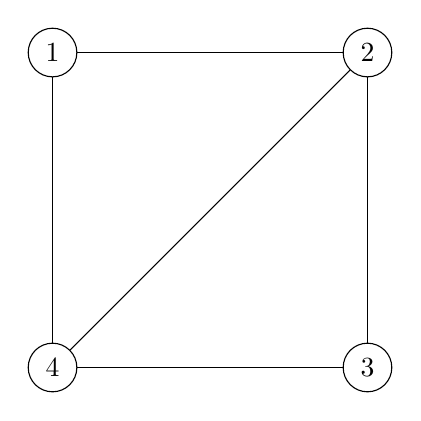
\begin{tikzpicture}[scale=2,auto=center,every node/.style={circle,draw=black}]
        \node (2) at (-1,1) {2};
        \node (1) at (-3,1) {1};
        \node (3) at (-1,-1) {3};
        \node (4) at (-3, -1) {4};

        \draw (1) -- (2);
        \draw (2) -- (3);
        \draw (3) -- (4);
        \draw (4) -- (1);
        \draw (2) -- (4);

    \end{tikzpicture}
    
\end{figure}
\begin{parts}
\part Compute the chromatic polynomial of $G$. \marksA{3 points}
\part Compute $\chi(G)$. \marksA{1 point}
\part Compute the number of 5-colorings of $G$. \marksA{1 point}
\end{parts}

\question Prove the following by induction on $n$:

\begin{parts}    
\part $p_{C_n}(\lambda) = (\lambda - 1)^n + (-1)^n(\lambda - 1)$, where $C_n$ is the cycle of $n$ vertices. (Ask the coords or look at the theory given for an example of $C_n$ if you're confused) \marksA{4 points}

\part If $T_n$ is any \textit{tree} of $n$ nodes, $p_{T_n}(\lambda) = \lambda(\lambda - 1)^{n-1}$ (a tree of $n$ vertices is a graph with $n-1$ edges with no cycles, and every node is an endpoint of at least 1 edge.) \marksA{4 points} 

\end{parts}

\question Prove that for any $n \geq 4$, two non-isomorphic graphs of $n$ nodes (graphs which cannot be the same if you rename the nodes) may have the same chromatic polynomial. (An explicit construction of both graphs is enough, you do not need to prove that they are not isomorphic.) \marksA{3 points}

\question Suppose you already know the chromatic polynomial of a graph with $n$ nodes, and its coefficients are stored in an array of size $n+1$. Write an algorithm to compute the chromatic number of the graph in $O(n \log n)$ time (you don't need to be too formal but there should be no ambiguity.) \marksA{4 points}

\question The \textit{Mycielskian} $\text{My}(G)$ of a graph $G = (V, E)$ is defined as follows:

\begin{itemize}
    \item Let $V = \{v_1, v_2 \cdots v_n\}$ and $E = \{e_1, e_2, \cdots e_m\}$.
    \item Let $W_1 = \{w_1, w_2 \cdots w_n\}$ (a new vertex set of size $n$)
    \item Let $E_1 = \bigcup_{e = \{v_i, v_j\} \in E}(\{\{v_i, w_j\}, \{w_i, v_j\}\})$
    \item Let $W_2 = \{x\}$ (another new vertex set of size 1)
    \item Let $E_2 = \{\{w_i, x\} | w_i \in W_1\}$
    \item $\text{My}(G) = (V \cup W_1 \cup W_2, E \cup E_1 \cup E_2))$
    
\end{itemize}

What can you say about $\chi(\text{My}(G))$ if you know $\chi(G)$? State the relation between both and reason why (again, no need to be too formal). \marksA{15 marks}

\end{questions}

$$\square \square \square \square \square \square \square \square \square \square \square \square \square \square \square $$
\end{document}

%https://www.dropbox.com/sh/w9mfy9qtjs68xzc/AAAOrtU5GcEmE01sbNoSDqzVa/Combinatorics/Generating%20Functions%20-%20Maria%20Monks%20-%20MOP%202010.pdf?dl=0